% Chapter 4

\chapter{Event Identity Information Management (EIIM) Life Cycle for Social Media} % Main chapter title

\label{eiim} % For referencing the chapter elsewhere, use \ref{Chapter1} 

\lhead{Chapter 4. \emph{Event Identity Information Management (EIIM) Life Cycle for Social Media}} % This is for the header on each page - perhaps a shortened title


%\section{Background : Entity Identity Information Management}



\begin{figure}[htbp]
  \caption{Identity Integrity component of the EIIM life cycle.}
  \centering
    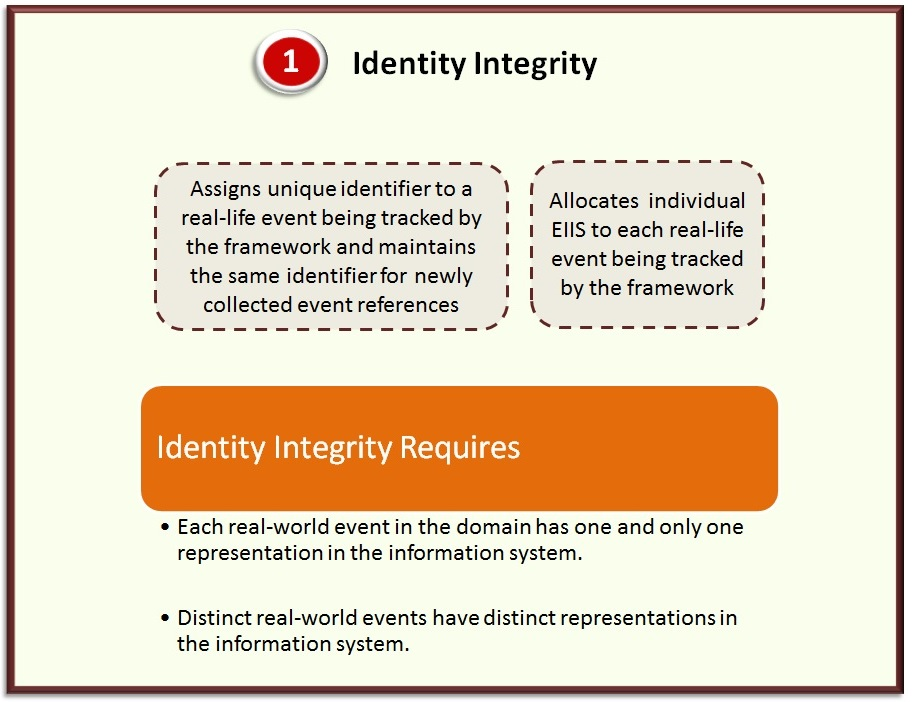
\includegraphics[width=14cm,height=11cm]{Figures/EIIMComponents/IdentityIntegrity.jpg}
\end{figure}

\section{Identity Integrity}
One of the fundamental goals of the proposed framework is to maintain a one-to-one correspondence between real-world events being monitored and the Event Identity Information Structure (EIIS) of the corresponding events for ensuring identity integrity. Therefore, a separate EIIS is maintained corresponding to each event. As new events are introduced to the framework, a unique identifier is assigned to them along with the allocation of individual EIIS structures. The framework is expected to maintain the integrity throughout the EIIM life cycle, by consistently assigning the same identifier to the references of a tracked event. Modules of this component assigns 12 byte unique integers known as ObjectId  to each event, and is also responsible for maintaining the same ObjectId for event ids of collected references and related EIIS. It is also the functionality of this component to assign the right identifier to the references resolved for an event by the Event Reference Resolution component.


\section{Event Reference Collection}

\begin{figure}[htbp]
  \caption{Event Reference Collection component of the EIIM life cycle.}
  \centering
    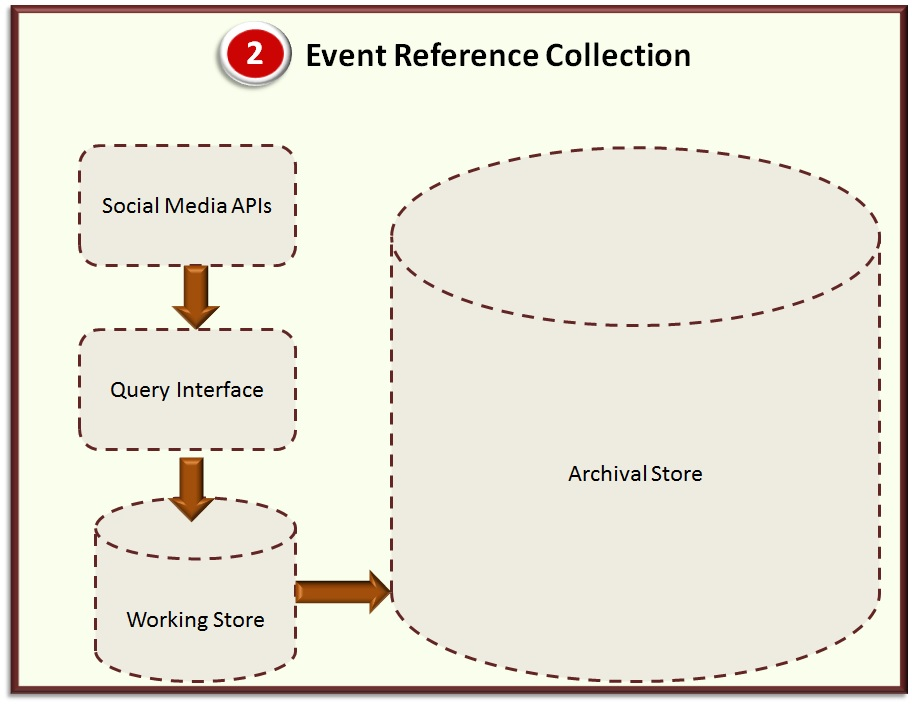
\includegraphics[width=14cm,height=11cm]{Figures/EIIMComponents/EventReferenceCollection.jpg}
\end{figure}

This component allows the framework to collect event references from different social media websites using its publicly available APIs (Application Programming Interface), and store them in the database after processing them using the next two components of the EIIM life cycle. Due to the semi-structured nature of the collected data, a NOSQL document oriented database management system (MongoDb ) is used for storage. The choice of MongoDb was also driven by its ability to scale horizontally and perform operations on large volumes of data.
For the experiments and analysis 4 million tweets (approx) related to five different events were collected using this component. Details of the collected event references are provided in Table 2. The tweets were collected over the given period of time, by providing a popular hashtag to the Twitter streaming API  (for details about Twitter Data Collection please refer Appendix \ref{AppendixA}.

\begin{table}[htbp]
\center
\caption{Details of data collected for analyzing event related tweet content.}
\label{informationcuedata}
\begin{tabular}{|c|c|c|c|}
\hline
\textbf{Event} & \textbf{Query Hashtag}                          & \shortstack{\textbf{No. of} \\ \textbf{Tweets}} & \shortstack{\textbf{Time Period}}                               \\ \hline
\shortstack{Sochi Winter\\ Games 2014 \\ ($http://goo.gl/sG4Rqd$)}& \#sochi2014 & 1958220 & \shortstack{11th Feb,2014\\ to\\ 3rd March, 2014} \\ \hline
\begin{tabular}[c]{@{}c@{}}SXSW 2014  \\ ($http://goo.gl/b6Nd6X$)\end{tabular} & sxsw2014                                  & 1880557                                                            & \begin{tabular}[c]{@{}c@{}}8th March, 2014\\ to\\ 16th March, 2014\end{tabular} \\ \hline
\begin{tabular}[c]{@{}c@{}}CPAC 2014 \\ ($http://goo.gl/9o1KUx$)\end{tabular} & \#cpac2014 & 18104                                                              & \begin{tabular}[c]{@{}c@{}}7th March, 2014\\ to\\ 16th March, 2014\end{tabular} \\ \hline
\shortstack{Millions March NYC \\ ($http://goo.gl/I8WR4B$)} & \#millionsmarchnyc  & 56927 & \shortstack{13th Dec, 2014\\ 20:25:43\\ to\\ 14th Dec, 2014\\ 03:30:41} \\ \hline
\begin{tabular}[c]{@{}c@{}}Sydney Siege \\ ($http://goo.gl/qLguvG$)\end{tabular} & \#sydneysiege                                  & 398204                                                            & \begin{tabular}[c]{@{}c@{}}15th Dec, 2014\\ 07:21:16\\ to\\ 15th Dec, 2014\\ 22:46:45\end{tabular} \\ \hline
\end{tabular}
\end{table} 


\section{Event Reference Preparation}

\begin{figure}[htbp]
  \caption{Event Reference Preparation component of the EIIM life cycle.}
  \centering
    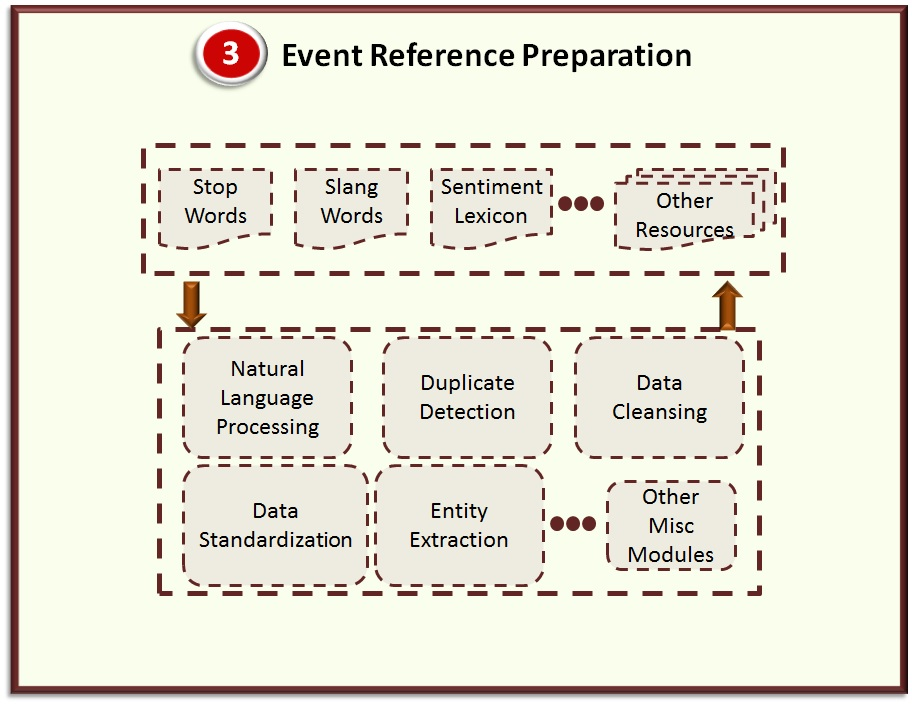
\includegraphics[width=14cm,height=11cm]{Figures/EIIMComponents/EventReferencePreparation.jpg}
\end{figure}

Preprocessing the raw references is an important stage of any data intensive application. This component performs a series of data preparation steps on the collected event tweets in order to make them suitable for further processing by the other components of the EIIM life cycle. It performs deduplication of tweets using md5 hashing scheme. Redundant copies of a tweet are filtered out keeping a single copy in the database. Parts-of-speech tagging is done using the default POS tagger available in the NLTK  module. A standard list of English stop words is used for eliminating the stop words from the tweet text. All the characters of a tweet are converted into lower case and special characters are removed. The tweets are tokenized into unigram tokens. User mentions, retweet symbol and URLs are removed during tokenization and are not considered as tokens.

A list of words expressing feelings in the internet, obtained from wefeelfine.org is used for detecting and extracting the feeling words from a tweet. Slang words commonly used in the internet and twitter specific slang publicly shared by FBI  is combined together for compiling a list of English slang words. The modules use this list for detecting and extracting the slang words from the tweets, hashtags and text units. Retweet counts, favorite counts, verification information, user follower count, time information and expanded form of the URLs shared in the tweets are extracted from the metadata associated with each tweet, as retrieved using the Twitter API. 


\section{Event Information Quality}

\begin{figure}[htbp]
  \caption{Event Information Quality component of the EIIM life cycle.}
  \centering
    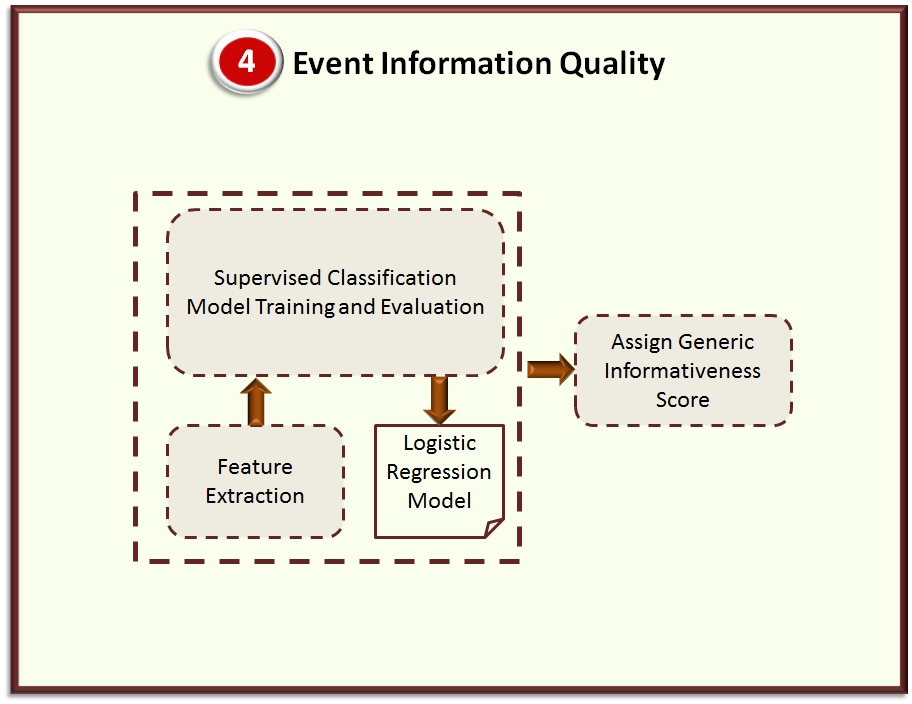
\includegraphics[width=14cm,height=11cm]{Figures/EIIMComponents/EventInformationQuality.jpg}
\end{figure}

This component examines the quality of information present in the tweets collected for the events. It segregates the references having high likelihood of containing good quality event related information from the ones that are less likely to contain or point to good quality information. In order to make a generic module for identifying high quality event related informative references we implemented a logistic regression classifier trained on a publicly available annotated dataset provided by [28]. The tweets labeled as ‘related and informative’ were assigned a score of 1 and all the other tweets labeled as ‘related-but not informative’, and ‘not related’ were assigned a score of 0. Table 3 lists the features extracted from each tweet. The choice of features was governed by previous works related to identifying high quality information from Twitter as already pointed in the Related Work section. 10-fold cross validation was performed resulting in a model with an accuracy of 76.64%. Table 4 lists the evaluation measures obtained while training the classifier.
The trained model is used for assigning a score between 0 (least informative) and 1 (most informative) to the tweets in real-time. Both the ‘Event Reference Preparation’ and the ‘Event Information Quality’ components work in collaboration with the ‘Event Reference Collection’ component in order to collect, prepare, assign quality score and store the tweets related to an event, obtained from Twitter streaming API, in real-time.

\begin{savenotes}
\begin{table}[ht]
\centering
\caption{Tweet features for content informativeness.}
\label{tweetfeature}
\begin{tabular}{|l|}
\hline
Has Url, No. of words, No. of stopwords, No. of feeling words, No. of slang \\ 
words, No. of hashtags, No. of user mentions, Tweet  length (No. of characters),\\  No. of unique 
characters, No. of special characters, Favorite count, Retweet \\ count, Formality, Is tweet verified, No. of nouns, No. of adjectives, No. of \\ verbs, No. of adverbs, No. of pronouns, No. of interjections, No. of articles, \\ No. of prepositions.
 \\ \hline
\end{tabular}
\end{table}
\end{savenotes}

\begin{table}[ht]
\centering
\caption{Evaluation measures for logistic regression model.}
\label{logregreseval}
\begin{tabular}{c|c|c|c|}
\cline{2-4}
\multicolumn{1}{l|}{}                          & \textbf{Precision} & \textbf{Recall}       & \textbf{F1-score}     \\ \hline
\multicolumn{1}{|c|}{\textbf{Non-informative} (0)} & 0.70               & 0.49                  & 0.57                  \\ \hline
\multicolumn{1}{|c|}{\textbf{Informative} (1)}     & 0.78               & 0.90                  & 0.84                  \\ \hline
\multicolumn{1}{|c|}{\textbf{Avg/Total}}       & 0.76               & 0.77                  & 0.75                  \\ \hline
\multicolumn{1}{|c}{\textbf{Accuracy}} =  & \multicolumn{1}{l}{} 76.64\%            & \multicolumn{1}{l}{} & \multicolumn{1}{l|}{} \\ \hline
\end{tabular}
\end{table}

\begin{figure}[htbp]
\centering
\caption{Content characteristics of informative and non-informative tweets related to events.}
    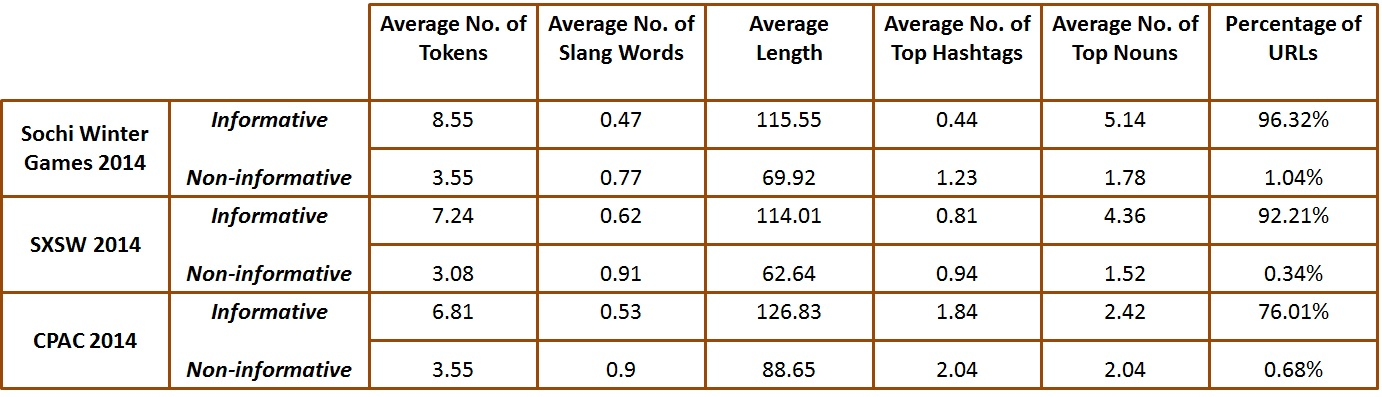
\includegraphics[width=15cm,height=5.5cm]{Figures/InformationAnalysisTable.jpg}
    
    \label{infoanalysis}
\end{figure}



\section{Event Identity Information Capture}

\begin{figure}[htbp]
  \caption{Event Identity Information Capture component of the EIIM life cycle.}
  \centering
    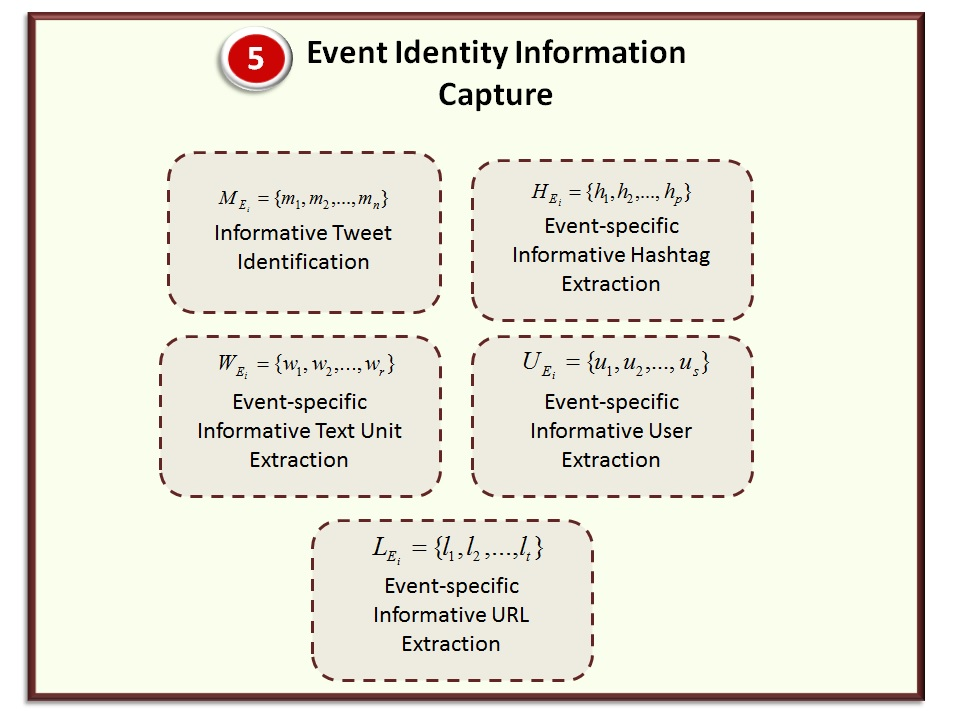
\includegraphics[width=14cm,height=11cm]{Figures/EIIMComponents/EventIdentityInformationCapture.jpg}
\end{figure}

It is the component that aids in extracting event identity information units (explained later) from the already processed tweets and build the Event Identity Information Structure (EIIS) for an event. It also enables the framework to set a threshold between 0.0-1.0 for differentiating between high quality informative tweets from low quality non-informative ones related to an event. The event identity information units are then extracted from the high quality informative tweets. 
In order to understand what might consist of the event identity information units that would represent the EIIS, we conducted a detailed analysis of 3.8 million tweets collected for three events. Details of the data collected are provided in Table 6. The data collection task was accomplished by Event Reference Collection component and was then preprocessed by the Event Reference Preparation component.

The logistic regression model developed for the Event Information Quality component was used for assigning scores to all the 3.8 million tweets in the dataset. The tweets getting a score greater than 0.7 were considered as instances of high quality informative tweets. Those getting a score lesser than 0.3 were considered as instances of low quality non-informative tweets. Average values of different content characteristics of the tweets were calculated. Top ten percent of the frequently occurring hashtags and nouns were considered as top hashtags and top nouns respectively, for the analysis. Some of the characteristics that were prominently different for informative and non-informative tweets are listed in Table 5.
As presented in the table, for all the three events, on an average the informative tweets are marked by a higher number of tokens per tweet and greater occurrence of top nouns. The average length of informative tweets is also more than the non-informative ones. The percentage of informative tweets having URLs is strikingly high. A greater use of slang words is observed in non-informative tweets. However, greater occurrence of top hashtags in non-informative tweets intrigued us to look into the content and obtain a detailed view of it. We observed that a lot of non-informative tweets have used popular hashtags with unrelated content and URLs directing to irrelevant information. This is typical of spam tweets as already reported by [30]. Although not shown due to space constraints, the average number of follower counts for users posting informative tweets was also observed to be higher than the ones posting non-informative ones. The average number of feeling words used in informative tweets were also relatively higher than the feeling words used in the non-informative tweets. 

The above observations gave us an idea of how high quality informative content related to events is produced in Twitter and the characteristics that differentiate them from low quality non- informative content. It is now intuitive that the informative tweets are more expressive, formal and lengthier, marked by higher presence of nouns. The high presence of nouns indicates that these tweets also contain information about people, places, organizations, etc, associated with the events, which is vital information about any event and is ideal for representing its identity. Due to the limitations imposed by Twitter on the number of characters in a tweet, the users tend to share URLs along with the textual content that might lead to more information about the event. Also, users with high follower counts tend to post informative tweets. This can also be concluded by the fact that as they have more followers they are encouraged to share informative content. Conversely, since they share informative content they are followed by a large number of other users interested in the content shared by them.
Based on the above analysis we decided to build the EIIS for an event composed of the following event identity information units:



\section{Event Identity Information Structure}

\begin{figure}[htbp]
  \caption{Event Identity Information Structure component of the EIIM life cycle.}
  \centering
    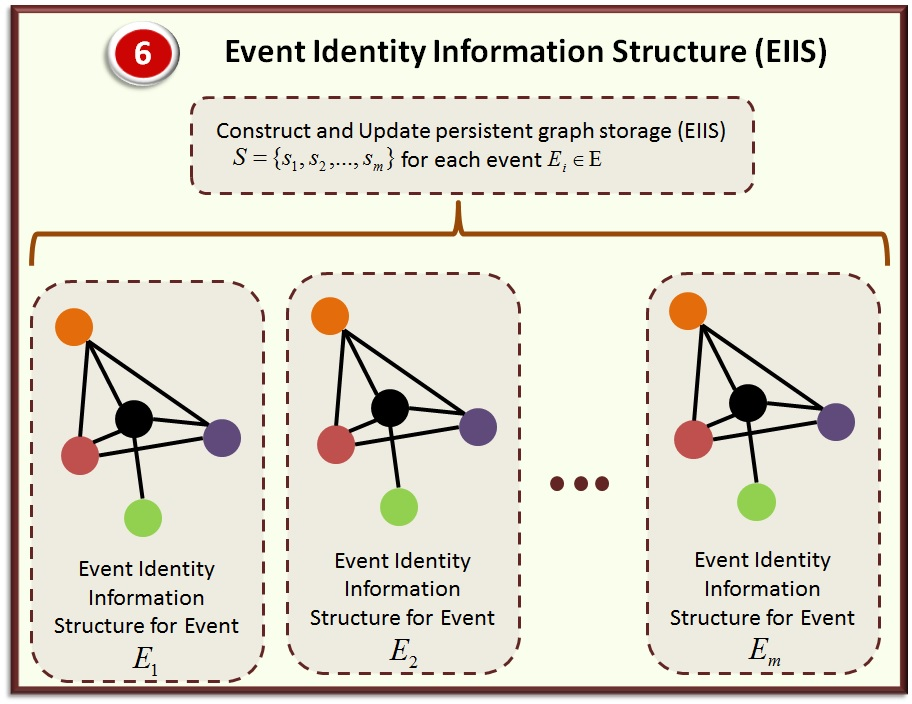
\includegraphics[width=14cm,height=11cm]{Figures/EIIMComponents/EventIdentityInformationStructure.jpg}
\end{figure}

\section{Event Identity Information Processing\label{EventIdentityInformationProcessing}}

\begin{figure}[htbp]
  \caption{Event Identity Information Processing component of the EIIM life cycle.}
  \centering
    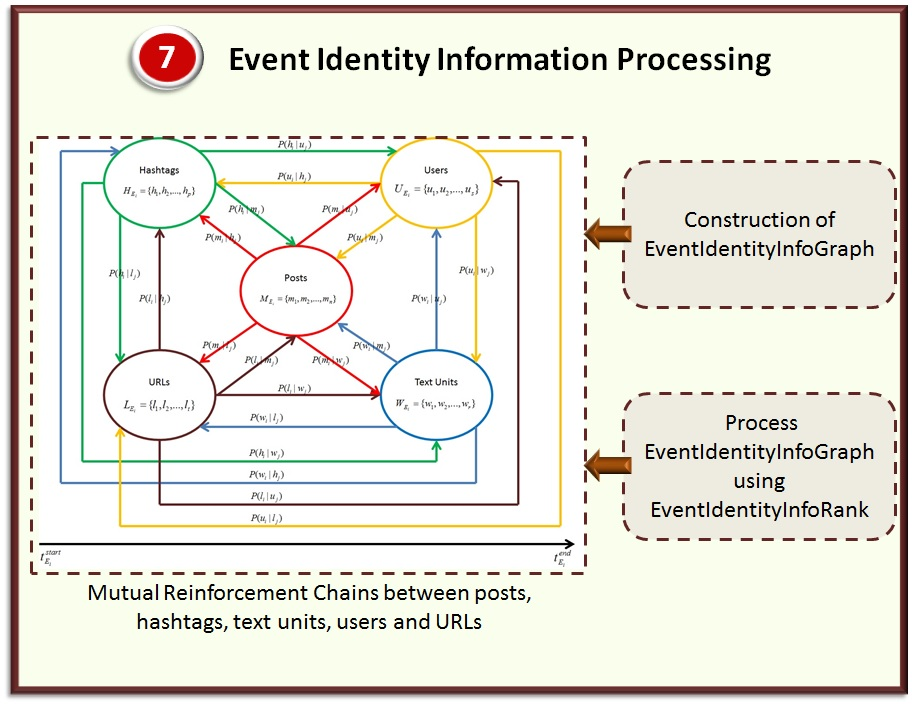
\includegraphics[width=14cm,height=11cm]{Figures/EIIMComponents/EventIdentityInformationProcessing.jpg}
\end{figure}


\begin{table*}[ht]
\caption{Affinity scores of edges between vertices of TwitterEventInfoGraph}
\label{edgescores}
\begin{tabular}{|l|}
\hline 
\underline{\textbf{\textit{Affinity scores (edge weights) between different vertices}} $\in M_{E_{i}}, H_{E_{i}}, W_{E_{i}}, U_{E_{i}},$} \\ \underline{\textbf{\textit{$L_{E_{i}}$:}}} \\ \\
$P(h_{i} \mid w_{j}) = \frac{No. \, of \, tweets \, h_{i} \, and \, w_{j} \, occur \, together}{No. \, of \, tweets \, w_{j} \, occurs}$, $P(w_{i} \mid h_{j}) = \frac{No. \, of \, tweets \, w_{i} \, and \, h_{j} \, occur \, together}{No. \, of \, tweets \, h_{j} \, occurs}$, \\


$P(h_{i} \mid l_{j}) = \frac{No. \, of \, tweets \, h_{i} \, and \, l_{j} \, occur \, together}{No. \, of \, tweets \, l_{j} \, occurs}$,
$P(l_{i} \mid h_{j}) = \frac{No. \, of \, tweets \, l_{i} \, and \, h_{j} \, occur \, together}{No. \, of \, tweets  \, h_{j} \, occurs}$, \\

$P(h_{i} \mid u_{j}) = \frac{No. \, of \, tweets  \, h_{i} \, and \, u_{j} \, occur \, together}{No. \, of \, tweets  \, u_{j} \, occurs}$,
$P(u_{i} \mid h_{j}) = \frac{No. \, of \, tweets  \, u_{i} \, and \, h_{j} \, occur \, together}{No. \, of \, tweets  \, h_{j} \, occurs}$,  \\

$P(w_{i} \mid l_{j}) = \frac{No. \, of \, tweets  \, w_{i} \, and \, l_{j} \, occur \, together}{No. \, of \, tweets  \, l_{j} \, occurs}$, 
$P(l_{i} \mid w_{j}) = \frac{No. \, of \, tweets  \, l_{i} \, and \, w_{j} \, occur \, together}{No. \, of \, tweets  \, w_{j} \, occurs}$, \\ 

$P(w_{i} \mid u_{j}) = \frac{No. \, of \, tweets  \, w_{i} \, and \, u_{j} \, occur \, together}{No. \, of \, tweets  \, u_{j} \, occurs}$,
$P(u_{i} \mid w_{j}) = \frac{No. \, of \, tweets  \, u_{i} \, and \, w_{j} \, occur \, together}{No. \, of \, tweets  \, w_{j} \, occurs}$, \\

$P(u_{i} \mid l_{j}) = \frac{No. \, of \, tweets  \, u_{i} \, and \, l_{j} \, occur \, together}{No. \, of \, tweets  \, l_{j} \, occurs}$, 
$P(l_{i} \mid u_{j}) = \frac{No. \, of \, tweets  \, l_{i} \, and \, u_{j} \, occur \, together}{No. \, of \, tweets  \, u_{j} \, occurs}$, \\


$P(h_{i} \mid m_{j}) = P(m_{i} \mid h_{j}) = P(w_{i} \mid m_{j}) = P(m_{i} \mid w_{j}) = P(u_{i} \mid m_{j}) = P(m_{i} \mid u_{j}) =$ \\ $P(l_{i} \mid m_{j})= P(m_{i} \mid l_{j})= 1.0$  \\ \\ 
\textbf{Note:} $P(h_{i} \mid w_{j})$ should be read as the probability of occurrence of hashtag $h_{i}$ given \\ the occurrence of the text unit $w_{j}$ in the stream of  tweets $M_{E_{i}}$ related to event $E_{i}$ \\ collected over the time period $T_{E_{i}}$. Similarly, for others.\\
\hline 
\end{tabular}
\end{table*}


\begin{figure}[htbp]
\centering
\caption{\small Mutual Reinforcement Chains in Twitter for an event.}    
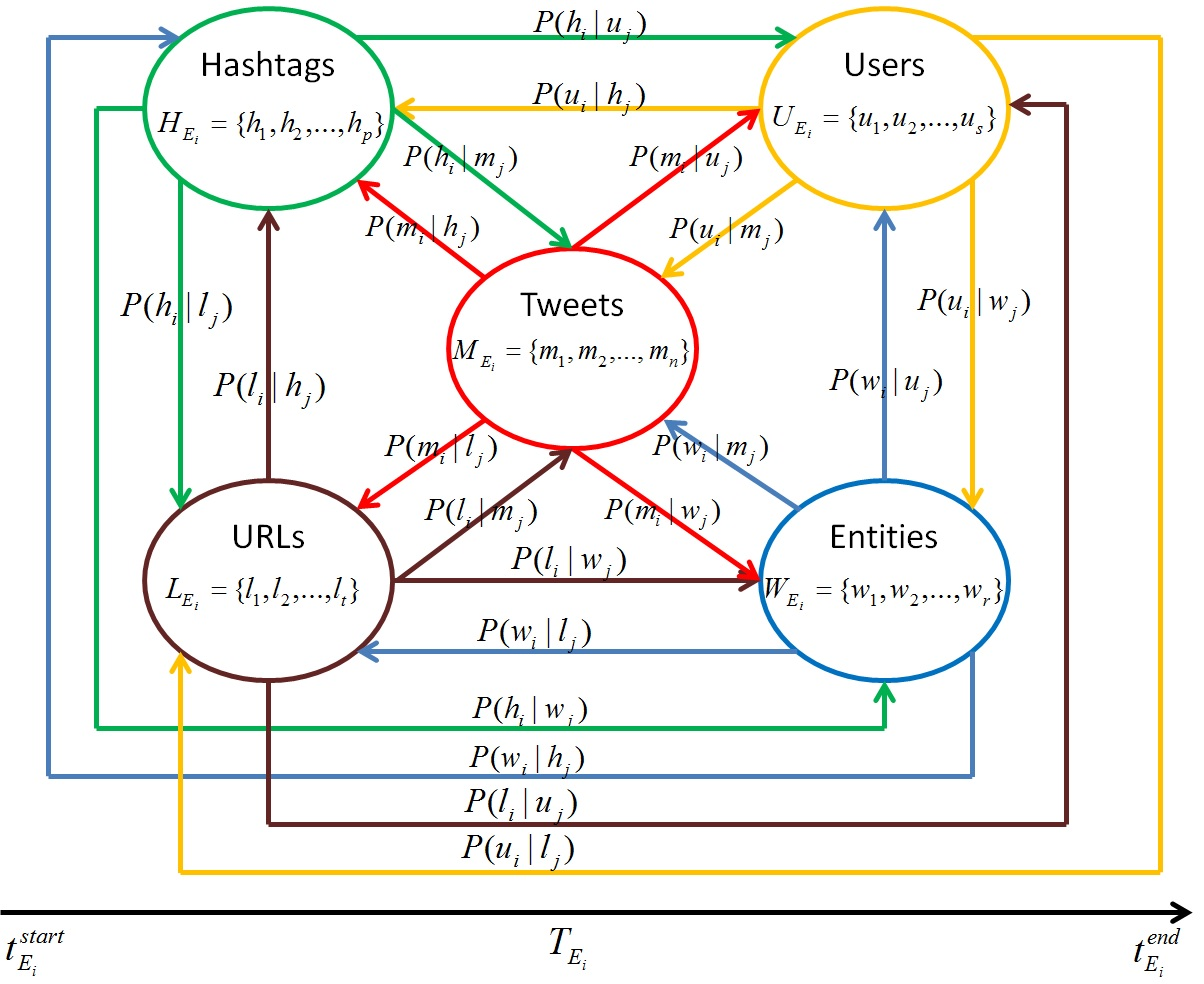
\includegraphics[width=16cm,height=12cm]{Figures/TwitterEventInfoGraph.jpg}
\label{mrc}
\end{figure}








For an event $E_{i}$ 
\begin{itemize} 
\item a \textit{tweet is an event-specific informative tweet} if it is strongly associated with:
\begin{itemize}
\item[\textbf{(a)}] \textit{event-specific informative hashtags}, 
\item[\textbf{(b)}] \textit{event-specific informative text units}, 
\item[\textbf{(c)}] \textit{event-specific informative users},
\item[\textbf{(d)}] \textit{event-specific informative URLs}. 
\end{itemize}
\end{itemize}

\begin{itemize} 
\item a \textit{hashtag is an event-specific informative hashtag} if it is strongly associated with:
\begin{itemize}
\item[\textbf{(a)}] \textit{event-specific informative tweets},
\item[\textbf{(b)}] \textit{event-specific informative text units},
\item[\textbf{(c)}] \textit{event-specific informative users},
\item[\textbf{(d)}] \textit{event-specific informative URLs}.
\end{itemize}
\end{itemize}

\begin{itemize} 
\item a \textit{text unit is an event-specific informative text unit} if it is strongly associated with:
\begin{itemize}
\item[\textbf{(a)}] \textit{event-specific informative tweets}, 
\item[\textbf{(b)}] \textit{event-specific informative hashtags}, 
\item[\textbf{(c)}] \textit{event-specific informative users}, 
\item[\textbf{(d)}] \textit{event-specific informative URLs}. 
\end{itemize}
\end{itemize}

\begin{itemize} 
\item a \textit{user is an event-specific informative user} if it is strongly associated with:
\begin{itemize}
\item[\textbf{(a)}] \textit{event-specific informative tweets}, 
\item[\textbf{(b)}] \textit{event-specific informative hashtags}, 
\item[\textbf{(c)}] \textit{event-specific informative text units},
\item[\textbf{(d)}] \textit{event-specific informative URLs}. 
\end{itemize}
\end{itemize}

\begin{itemize} \item a \textit{URL is an event-specific informative URL} if it is strongly associated with:
\begin{itemize}
\item[\textbf{(a)}] \textit{event-specific informative tweets}, 
\item[\textbf{(b)}] \textit{event-specific informative hashtags}, 
\item[\textbf{(c)}] \textit{event-specific informative text units},
\item[\textbf{(d)}] \textit{event-specific informative users}. 
\end{itemize}
\end{itemize}

%\end{itemize}

The relationships for an event $\scriptstyle E_{i}$ as stated above, forms a \textit{Mutual Reinforcement Chain} \cite{wei2008query} for the event $E_{i}$ as shown in Figure \ref{mrc}. We represent this relationship in a graph $\textbf{G = (V,D)}$, which we call as \textit{TwitterEventInfoGraph}, where $\mathbf{V = M_{E_{i}} \cup H_{E_{i}} \cup W_{E_{i}} \cup U_{E_{i}} \cup L_{E_{i}}}$, is the set of vertices and $\mathbf{D}$ is the set of directed edges between different vertices. 

Whenever two vertices are associated, there are two edges between them that are oppositely directed. Each directed edge is assigned a weight, which determines the degree of association of one vertex with the other. The weights for each edge is calculated according to the conditional probabilities given in Table \ref{edgescores}. 

We do not consider an edge between two vertices of same type. That is, we don't connect a tweet with another tweet. Similarly, for hashtags, text units, users and URLs. This constraint was imposed in order to deal with the nepotistic relationships between high quality content and low quality content introduced by the malicious users for promoting the low quality content. We observe these malicious side effects in the results obtained for \textit{TextRank} explained in Section 6.5.  

Next, we explain \textit{TwitterEventInfoRank}.

%%%%%%%%%%%%%%%%%%%%%%%%%%%%%%%%%%%%%%%%%%%%%%%%%%%%%%%%%%%%%%%%%%%%%%%%%%%%%%%%%%
%%%%%%%%%%%%%%%%%                                       TwitterEventInfoRank Subsection                    %%%%%%%%%%%%%%%%%%%%%%%%%%%%%%%%%%
%%%%%%%%%%%%%%%%%%%%%%%%%%%%%%%%%%%%%%%%%%%%%%%%%%%%%%%%%%%%%%%%%%%%%%%%%%%%%%%%%%

\subsection{TwitterEventInfoRank\label{twitterEventInfoRank}}
In this section, we introduce an iterative algorithm that takes into account the mutually reinforcing relationships between the vertices of \textit{TwitterEventInfoGraph} as explained in the previous section and propagates event-specific scores of each vertex to connected vertices across the graph for ranking its vertices ($\scriptstyle \in V$) in terms of event-specific informativeness.

We first assign a event-specific score to all the vertices of the graph. Event-specific scores for vertices $(\in H_{E_{i}}, W_{E_{i}}, U_{E_{i}}, L_{E_{i}})$ are calculated using equations (1-4) as presented in Table \ref{edgescores}. The tweets  $(\in M_{E_{i}})$ are assigned an initial informativeness score as obtained from the logistic regression model explained in Section 3. The event-specific scores for vertices $(\in H_{E_{i}}, W_{E_{i}}, U_{E_{i}}, L_{E_{i}})$ and informativeness score for vertices $(\in M_{E_{i}})$ gives an initial ranking of all the vertices of \textit{TwitterEventInfoGraph}. We aim to refine the initial scores and assign a final score for ranking the vertices by leveraging the mutually reinforcing relationships between them.
\begin{equation}
Score(h_{i}) = \frac{freq(h_{i})}{max\{freq(h_{1}),freq(h_{2}),...,freq(h_{p})\}}
\end{equation}

\begin{equation}
Score(w_{i}) = \frac{freq(w_{i})}{max\{freq(w_{1}),freq(w_{2}),...,freq(w_{r})\}}
\end{equation}

\begin{equation}
Score(u_{i}) = \frac{followers(u_{i})}{max\{followers(u_{1}),...,followers(u_{r})\}}
\end{equation}

\begin{equation}
Score(l_{i}) = \frac{freq(l_{i})}{max\{freq(l_{1}),freq(l_{2}),...,freq(l_{r})\}}
\end{equation}


The relationships between two different subsets of vertices in graph $\scriptstyle \mathbf{G}$ is denoted by an affinity matrix. For e.g., $\mathbf{A_{E_{i}}^{MH}}$ denotes the $\mathbf{M_{E_{i}}-H_{E_{i}}}$ affinity matrix for event $E_{i}$, where $\mathbf{(i,j)^{th}}$ entry is the edge weight quantifying the association between $i^{th}$ tweet ($\in M_{E_{i}}$) and $j^{th}$ hashtag ($\in H_{E_{i}}$), calculated using Table \ref{edgescores}. Similarly, $\mathbf{A_{E_{i}}^{WH}}$ denotes the $\mathbf{W_{E_{i}}-H_{E_{i}}}$ affinity matrix between set of text units $W_{E_{i}}$ and set of hashtags $H_{E_{i}}$ for event $E_{i}$, and so on.


The rankings of \textit{tweets}, \textit{hashtags}, \textit{text units}, \textit{users} and \textit{URLs} in terms of event-specific informativeness, can be iteratively derived from the Mutual Reinforcement Chain for the event. Let $R_{{E_{i}}}^{M}$, $R_{{E_{i}}}^{H}$, $R_{{E_{i}}}^{W}$, $R_{{E_{i}}}^{U}$ and $\scriptstyle R_{{E_{i}}}^{L}$ denote the ranking scores for the set of tweets ($\in M_{E_{}}$), set of  hashtags $(\in H_{E_{i}})$, set of text units $(\in W_{E_{i}})$, set of users $(\in U_{E_{i}})$, and set of URLs $(\in L_{E_{i}})$, respectively. Therefore, the Mutual Reinforcement Chain ranking for the $k^{th}$ iteration can be formulated as follows:
 

%\begin{equation}
%\tiny R_{{E_{i}}}^{M(k+1)} = A_{E_{i}}^{MM(k)}R_{{E_{i}}}^{M(k)} + A_{E_{i}}^{MH(k)}R_{{E_{i}}}^{H(k)} + A_{E_{i}}^{MW(k)}R_{{E_{i}}}^{W(k)} + A_{E_{i}}^{MU(k)}R_{{E_{i}}}^{U(k)} + A_{E_{i}}^{ML(k)}R_{{E_{i}}}^{L(k)}
%\end{equation}

\begin{equation}
R_{{E_{i}}}^{M(k+1)} = A_{E_{i}}^{MM(k)}R_{{E_{i}}}^{M(k)} + A_{E_{i}}^{MH(k)}R_{{E_{i}}}^{H(k)} + A_{E_{i}}^{MW(k)}R_{{E_{i}}}^{W(k)}+ A_{E_{i}}^{MU(k)}R_{{E_{i}}}^{U(k)} + A_{E_{i}}^{ML(k)}R_{{E_{i}}}^{L(k)}
\end{equation}

%\begin{equation}
%\tiny R_{{E_{i}}}^{H(k+1)} = A_{E_{i}}^{HM(k)}R_{{E_{i}}}^{M(k)} + A_{E_{i}}^{HH(k)}R_{{E_{i}}}^{H(k)} + A_{E_{i}}^{HW(k)}R_{{E_{i}}}^{W(k)} + A_{E_{i}}^{HU(k)}R_{{E_{i}}}^{U(k)} + A_{E_{i}}^{HL(k)}R_{{E_{i}}}^{L(k)}
%\end{equation}

\begin{equation}
R_{{E_{i}}}^{H(k+1)} = A_{E_{i}}^{HM(k)}R_{{E_{i}}}^{M(k)} + A_{E_{i}}^{HH(k)}R_{{E_{i}}}^{H(k)} + A_{E_{i}}^{HW(k)}R_{{E_{i}}}^{W(k)}+ A_{E_{i}}^{HU(k)}R_{{E_{i}}}^{U(k)} + A_{E_{i}}^{HL(k)}R_{{E_{i}}}^{L(k)}
\end{equation}



%\begin{equation}
%\tiny R_{{E_{i}}}^{W(k+1)} = A_{E_{i}}^{WM(k)}R_{{E_{i}}}^{M(k)} + A_{E_{i}}^{WH(k)}R_{{E_{i}}}^{H(k)} + A_{E_{i}}^{WW(k)}R_{{E_{i}}}^{W(k)} + A_{E_{i}}^{WU(k)}R_{{E_{i}}}^{U(k)} + A_{E_{i}}^{WL(k)}R_{{E_{i}}}^{L(k)}
%\end{equation}

\begin{equation}
R_{{E_{i}}}^{W(k+1)} = A_{E_{i}}^{WM(k)}R_{{E_{i}}}^{M(k)} + A_{E_{i}}^{WH(k)}R_{{E_{i}}}^{H(k)} + A_{E_{i}}^{WW(k)}R_{{E_{i}}}^{W(k)}+ A_{E_{i}}^{WU(k)}R_{{E_{i}}}^{U(k)} + A_{E_{i}}^{WL(k)}R_{{E_{i}}}^{L(k)}
\end{equation}

%\begin{equation}
%\tiny R_{{E_{i}}}^{U(k+1)} = A_{E_{i}}^{UM(k)}R_{{E_{i}}}^{M(k)} + A_{E_{i}}^{UH(k)}R_{{E_{i}}}^{H(k)} + A_{E_{i}}^{UW(k)}R_{{E_{i}}}^{W(k)} + A_{E_{i}}^{UU(k)}R_{{E_{i}}}^{U(k)} + A_{E_{i}}^{UL(k)}R_{{E_{i}}}^{L(k)}
%\end{equation}

\begin{equation}
R_{{E_{i}}}^{U(k+1)} = A_{E_{i}}^{UM(k)}R_{{E_{i}}}^{M(k)} + A_{E_{i}}^{UH(k)}R_{{E_{i}}}^{H(k)} + A_{E_{i}}^{UW(k)}R_{{E_{i}}}^{W(k)}+ A_{E_{i}}^{UU(k)}R_{{E_{i}}}^{U(k)} + A_{E_{i}}^{UL(k)}R_{{E_{i}}}^{L(k)}
\end{equation}

%\begin{equation}
%\tiny R_{{E_{i}}}^{L(k+1)} = A_{E_{i}}^{LM(k)}R_{{E_{i}}}^{M(k)} + A_{E_{i}}^{LH(k)}R_{{E_{i}}}^{H(k)} + A_{E_{i}}^{LW(k)}R_{{E_{i}}}^{W(k)} + A_{E_{i}}^{LU(k)}R_{{E_{i}}}^{U(k)} + A_{E_{i}}^{LL(k)}R_{{E_{i}}}^{L(k)}
%\end{equation}


\begin{equation}
R_{{E_{i}}}^{L(k+1)} = A_{E_{i}}^{LM(k)}R_{{E_{i}}}^{M(k)} + A_{E_{i}}^{LH(k)}R_{{E_{i}}}^{H(k)} +A_{E_{i}}^{LW(k)}R_{{E_{i}}}^{W(k)}+ A_{E_{i}}^{LU(k)}R_{{E_{i}}}^{U(k)}+ A_{E_{i}}^{LL(k)}R_{{E_{i}}}^{L(k)}
\end{equation}


The equations 5-9 can be represented in the form of a block matrix $\Delta_{E_{i}}$, where,
\[ \Delta_{E_{i}} = \left( \begin{array}{ccccc}
A_{E_{i}}^{MM} & A_{E_{i}}^{MH} & A_{E_{i}}^{MW} &  A_{E_{i}}^{MU} & A_{E_{i}}^{ML} \\
A_{E_{i}}^{HM} & A_{E_{i}}^{HH} & A_{E_{i}}^{HW} & A_{E_{i}}^{HU} & A_{E_{i}}^{HL} \\
A_{E_{i}}^{WM} & A_{E_{i}}^{WH} & A_{E_{i}}^{WW} & A_{E_{i}}^{WU} & A_{E_{i}}^{WL}\\
A_{E_{i}}^{UM} & A_{E_{i}}^{UH} & A_{E_{i}}^{UW} & A_{E_{i}}^{UU} & A_{E_{i}}^{UL} \\
A_{E_{i}}^{LM} & A_{E_{i}}^{LH} & A_{E_{i}}^{LW} & A_{E_{i}}^{LU} & A_{E_{i}}^{LL} \end{array} \right)\] 

Let \[R_{E_{i}} = \left( \begin{array}{c}
R_{{E_{i}}}^{M} \\
R_{{E_{i}}}^{H} \\
R_{{E_{i}}}^{W} \\
R_{{E_{i}}}^{U} \\
R_{{E_{i}}}^{L} \end{array} \right)\] 

then, $R_{E_{i}}$ can be computed as the dominant eigenvector of $\Delta_{E_{i}}$.
\begin{equation}
\Delta_{E_{i}}.R_{E_{i}} = \lambda.R_{E_{i}}
\end{equation}

In order to guarantee a unique $R_{E_{i}}$, $\Delta_{E_{i}}$ must be forced to be stochastic and irreducible. 

To make $\Delta_{E_{i}}$ stochastic we divide the value of each element in a column of $\Delta_{E_{i}}$ by the sum of the values of all the elements in that column. This finally makes $\Delta_{E_{i}}$ column stochastic. We now denote it by $\hat \Delta_{E_{i}}$.
%we remove all the rows and columns of the block matrices whose all elements are zeros. Since, we don't consider edges between two vertices of same type, all the elements of the diagonal block matrices are zero by default. We then 

Next, we make $\hat \Delta_{E_{i}}$ irreducible. This is done by making the graph $G$ strongly connected by adding links from one node to any other node with a probability vector $p$. Now, $\hat \Delta_{E_{i}}$ is transformed to 

\begin{equation}
\overline \Delta_{E_{i}} = \alpha \hat \Delta_{E_{i}} + (1-\alpha)E
\end{equation}
\begin{equation}
E = p \times [1]_{1 \times k}
\end{equation}
where $0 \le \alpha \le 1$ is set to 0.85 according to \textit{PageRank}, and k is the order of $\hat \Delta_{E_{i}}$. We set $p = [1/k]_{k \times 1}$ by assuming a uniform distribution over all elements. Now, $\overline \Delta_{E_{i}}$ is stochastic and irreducible and it can be shown that it is also primitive by checking $\overline \Delta_{E_{i}}^{2}$ is greater than $0$.

Following steps are taken next,
\begin{itemize}
\item[\textbf{1.}] We initialize the rank vectors ($ R_{{E_{i}}}^{M(0)}, R_{{E_{i}}}^{H(0)}, R_{{E_{i}}}^{W(0)}, R_{{E_{i}}}^{U(0)}, R_{{E_{i}}}^{L(0)}$) for each subset of vertices ($M_{E_{i}}, H_{E_{i}}, W_{E_{i}}, U_{E_{i}}, L_{E_{i}}$). We use the event-specific scores calculated for the set of hashtags, text units, users and urls as their initial scores. All the scores lie between 0 and 1. For the tweets we use the logistic regression model and assign each one of them an initial informativeness score between 0 and 1.

\item[\textbf{2.}] Then we assign
\[ R_{E_{i}}^{0} = \left( \begin{array}{c}
R_{{E_{i}}}^{M(0)} \\
R_{{E_{i}}}^{H(0)} \\
R_{{E_{i}}}^{W(0)} \\
R_{{E_{i}}}^{U(0)} \\
R_{{E_{i}}}^{L(0)} \end{array} \right)\] 

and normalize $R_{E_{i}}^{0}$ such that $\mid \mid R_{E_{i}}^{0}\mid \mid_{1} = 1$

\item[\textbf{3.}] Apply power iteration method using the same parameters as used in PageRank with the convergence tolerance set at 1e-08 and $\lambda = 0.85$ .

\item[\textbf{4.}] We get the final rank vectors for each subset of the vertices ($R_{{E_{i}}}^{M}, R_{{E_{i}}}^{H}, R_{{E_{i}}}^{W}, R_{{E_{i}}}^{U}, R_{{E_{i}}}^{L}$) after convergence. 

\item[\textbf{5.}] We finally obtain the subsets $\hat{M}_{E_{i}}, \hat{H}_{E_{i}}, \hat{W}_{E_{i}}, \hat{L}_{E_{i}}, \hat{U}_{E_{i}}$ consisting of the \textit{tweets}, \textit{hashtags}, \textit{text units}, \textit{URLs} and \textit{users}, respectively arranged in descending order of their final scores.

\end{itemize}

The final ordered subsets $\scriptstyle \mathbf{\hat{M}_{E_{i}}, \hat{H}_{E_{i}}, \hat{W}_{E_{i}}, \hat{L}_{E_{i}}, \hat{U}_{E_{i}}}$,  thus obtained are the tweets, hashtags, text units, URLs and users, ranked in terms of their event-specific informativeness. 

\begin{algorithm}
\label{algo}
\SetKwData{Left}{left}\SetKwData{This}{this}\SetKwData{Up}{up}
\SetKwFunction{Union}{Union}\SetKwFunction{FindCompress}{FindCompress}
\SetKwInOut{Input}{Input}\SetKwInOut{Output}{Output}
\Input{Sets of vertices $M_{E_{i}},H_{E_{i}}, W_{E_{i}}, U_{E_{i}}, L_{E_{i}}$ of graph G, $\alpha=0.85$, $\varepsilon=1e-08$.}
\BlankLine
\Output{Ordered set of vertices $\hat{M}_{E_{i}}$, containing tweets ranked in order of event-specific informative content sharing information about event related entities.}
\BlankLine
\textbf{Steps:}
\BlankLine
Initialize rank vectors $[R_{{E_{i}}}^{M(0)}, R_{{E_{i}}}^{H(0)}, R_{{E_{i}}}^{W(0)}, R_{{E_{i}}}^{U(0)}, R_{{E_{i}}}^{L(0)}]$\;
\BlankLine
Assign $R_{E_{i}}^{0}=[R_{E_{i}}^{M(0)},R_{E_{i}}^{H(0)},R_{E_{i}}^{W(0)},R_{E_{i}}^{U(0)},R_{E_{i}}^{L(0)}]^{T} $\;
\BlankLine
Normalize $R_{E_{i}}^{0}$ such that $\mid \mid R_{E_{i}}^{0}\mid \mid_{1} = 1$ \;
\BlankLine
Construct matrix $\Delta_{E_{i}}$\;
\BlankLine
Make matrix $\Delta_{E_{i}}$ stochastic and irreducible converting it to $\overline \Delta_{E_{i}}$\;
\BlankLine
$k \leftarrow 1$ 
\BlankLine
\Repeat{$\mid \mid R_{E_{i}}^{k} - R_{E_{i}}^{k-1} \mid \mid_{1} < \varepsilon \; OR \; k \ge 100$}{$R_{E_{i}}^{k} \leftarrow \overline \Delta_{E_{i}}R_{E_{i}}^{k-1}$\;
$k \leftarrow k+1$\; }
\BlankLine
$R_{E_{i}}^{M} \leftarrow R_{E_{i}}^{M(k)}$, $R_{E_{i}}^{H} \leftarrow R_{E_{i}}^{H(k)}$, $R_{E_{i}}^{W} \leftarrow R_{E_{i}}^{W(k)}$,  $R_{E_{i}}^{U} \leftarrow R_{E_{i}}^{U(k)}$, $R_{E_{i}}^{L} \leftarrow R_{E_{i}}^{L(k)}$\;
\BlankLine
$\hat{M}_{E_{i}} \leftarrow R_{E_{i}}^{M}$, $\hat{H}_{E_{i}} \leftarrow R_{E_{i}}^{H}$, $\hat{W}_{E_{i}} \leftarrow R_{E_{i}}^{W}$, $\hat{U}_{E_{i}} \leftarrow R_{E_{i}}^{U}$, $\hat{L}_{E_{i}} \leftarrow R_{E_{i}}^{L}$\;
\BlankLine
return $\hat{M}_{E_{i}}$,$\hat{H}_{E_{i}}$,$\hat{W}_{E_{i}}$,$\hat{U}_{E_{i}}$,$\hat{L}_{E_{i}}$\;
%\caption{\scriptsize Algorithm for ranking the nodes of G}\label{algo_disjdecomp}
\end{algorithm}\DecMargin{1em}

During the implementation of the \textit{TwitterEventInfoRank} algorithm the slang hashtags were removed. We only considered nouns as the text units and removed the slang words. We already reported in our analysis that non-informative tweets have higher slang content. Therefore, removal of slang hashtags and text units was done in order to obtain high quality results. We also showed higher occurrence of nouns in informative tweets. Also, the occurrence of a noun in a tweet intuitively suggests that the tweet has information about a person, place, or thing. Thus, we only considered the set of nouns extracted from the tweets as the set of text units. 

The text units are generic units in the framework and can be changed according to specific requirements. Entities extracted from the textual content of tweets could be experimented, in place of nouns. Since the algorithm uses power iteration method for ranking the vertices of the graph, it could be easily made scalable using mapreduce paradigm \cite{lin2010design}. We plan to work on it in the future and implement our framework using hadoop and mapreduce environment. 

Since, our proposed framework takes a hybrid approach by using both supervised and unsupervised component, it is easily applicable in situations where an event needs to be tracked over time. The supervised portion assigns an initial generic informativeness score to the tweets for bootstrapping an unsupervised process that finally assigns event-specific informativeness scores. When applied over a time period the method for assigning the initial supervised scores might remain the same and the unsupervised process can change the rankings of the tweet contents as the event evolves. 



\begin{figure}[htbp]
\centering
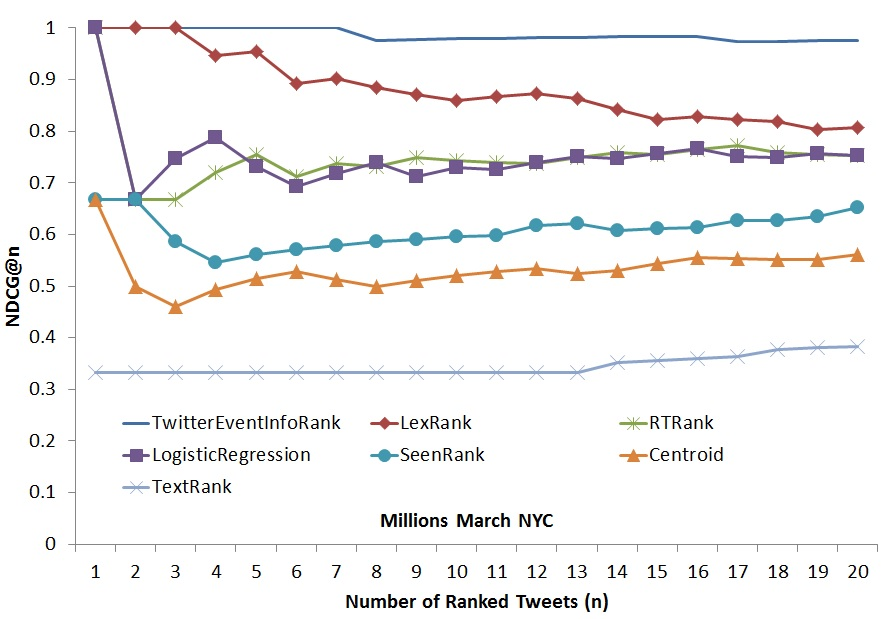
\includegraphics[height=4.5in,width=6in]{Figures/Chapter4Figures/MillionsMarchNycEventIdentityInfoRankPerformance.jpg}
\caption{\small Performance comparison of ranking techniques using NDCG scores.}
\label{millionsmarchndcg}
\end{figure}

\begin{figure}[htbp]
\centering
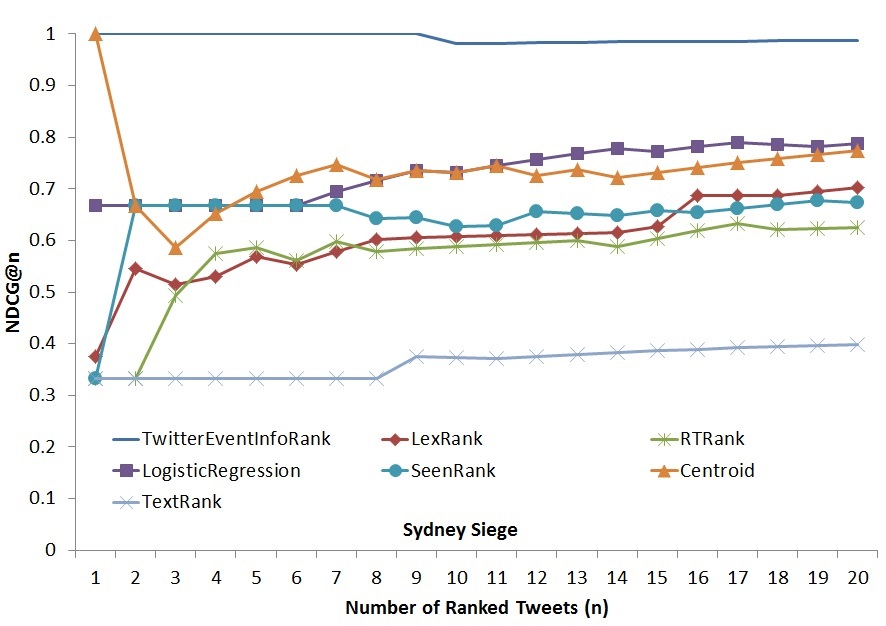
\includegraphics[height=4.5in,width=6in]{Figures/Chapter4Figures/SydneySiegeEventIdentityInfoRankPerformance.jpg}
\caption{\small Performance comparison of ranking techniques using NDCG scores.}
\label{sydneysiegendcg}
\end{figure}


\begin{table}[htbp]
\centering
\caption{Avg IIC scores and total avg scores of annotations for Millions March NYC event.}
\label{avgiicMillionsMarchNyc}
\begin{tabular}{|c|c|c|}
\hline
\textbf{\begin{tabular}[c]{@{}c@{}}Millions March \\ NYC\end{tabular}} & \textbf{IIC} & \textbf{\begin{tabular}[c]{@{}c@{}}Total Avg \\ Score (1-3)\end{tabular}} \\ \hline
\textbf{\begin{tabular}[c]{@{}c@{}}Top 50 event-specific\\ informative Hashtags\end{tabular}} & 0.786 & 1.980 \\ \hline
\textbf{\begin{tabular}[c]{@{}c@{}}Top 50 event-specific\\ informative Text Units\end{tabular}} & 0.880 & 1.320 \\ \hline
\textbf{\begin{tabular}[c]{@{}c@{}}Top 50 event-specific\\ informative URLs\end{tabular}} & 0.926 & 2.560 \\ \hline
\textbf{\begin{tabular}[c]{@{}c@{}}Top 50 event-specific\\ informative Users\end{tabular}} & 0.700 & 2.386 \\ \hline
\textbf{\begin{tabular}[c]{@{}c@{}}Top 100 event-specific\\ informative Tweets\end{tabular}} & 0.760 & 2.59 \\ \hline
\end{tabular}
\end{table}



\begin{table}[htbp]
\centering
\caption{Avg IIC scores and total avg scores of annotations for Sydney Siege event.}
\label{avgiicSydneySiege}
\begin{tabular}{|c|c|c|}
\hline
\textbf{Sydney Siege} & \textbf{IIC} & \textbf{\begin{tabular}[c]{@{}c@{}}Total Avg\\ Score (1-3)\end{tabular}} \\ \hline
\textbf{\begin{tabular}[c]{@{}c@{}}Top 50 event-specific\\ informative Hashtags\end{tabular}} & 0.880 & 2.027 \\ \hline
\textbf{\begin{tabular}[c]{@{}c@{}}Top 50 event-specific\\ informative Text Units\end{tabular}} & 0.986 & 1.487 \\ \hline
\textbf{\begin{tabular}[c]{@{}c@{}}Top 50 event-specific\\ informative URLs\end{tabular}} & 0.893 & 2.413 \\ \hline
\textbf{\begin{tabular}[c]{@{}c@{}}Top 50 event-specific\\ informative Users\end{tabular}} & 0.646 & 2.353 \\ \hline
\textbf{\begin{tabular}[c]{@{}c@{}}Top 100 event-specific\\ informative Tweets\end{tabular}} & 0.83 & 2.62 \\ \hline
\end{tabular}
\end{table}

\begin{figure}[htbp]
\centering
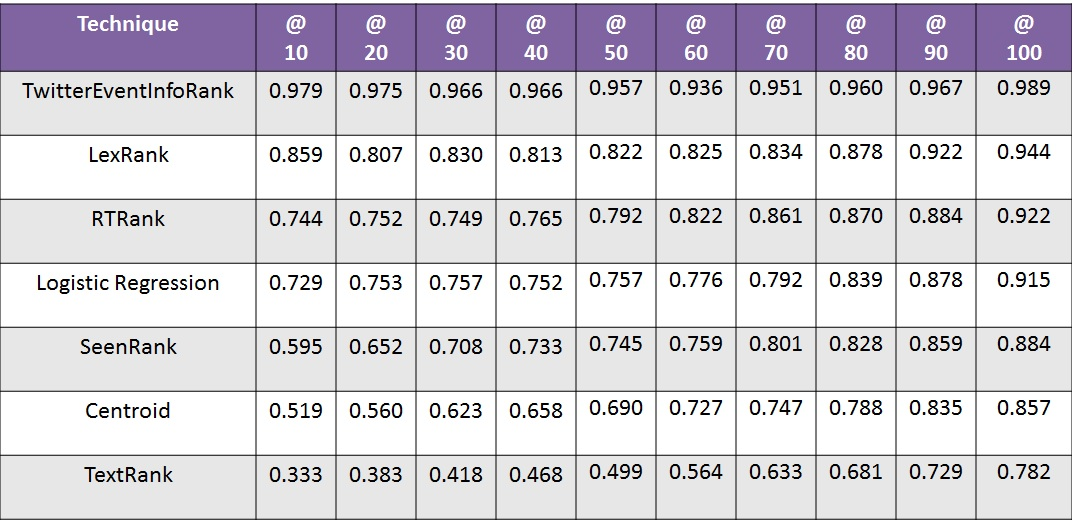
\includegraphics[height=3.5in,width=5.5in]{Figures/millionsmarchnycndcg.jpg}
\caption{\small Performance comparison of ranking techniques using NDCG scores.}
\label{millionsmarchndcg}
\end{figure}

\begin{figure}[htbp]
\centering
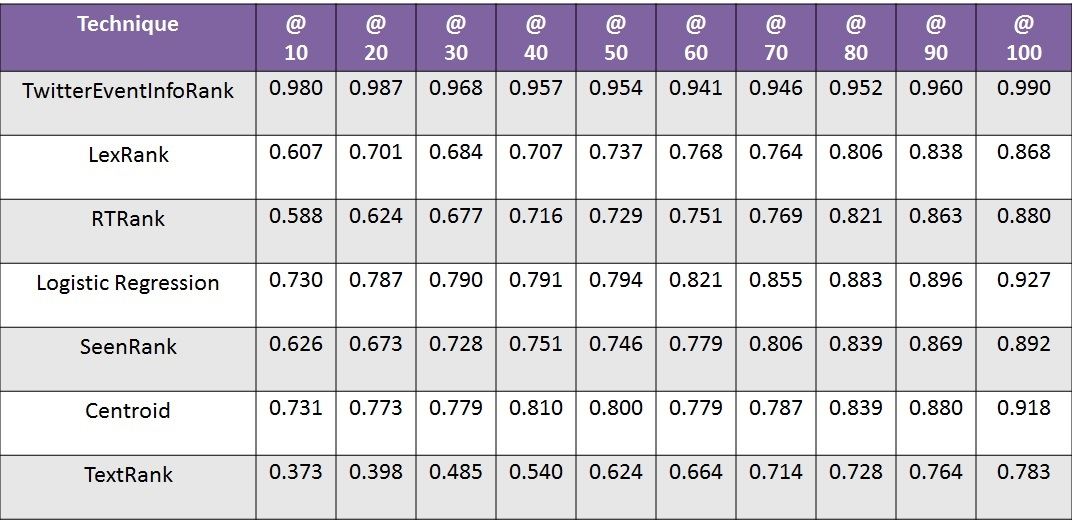
\includegraphics[height=3.5in,width=5.5in]{Figures/sydneysiegendcg.jpg}
\caption{\small Performance comparison of ranking techniques using NDCG scores.}
\label{sydneysiegendcg}
\end{figure}

\begin{figure}[htbp]
\centering
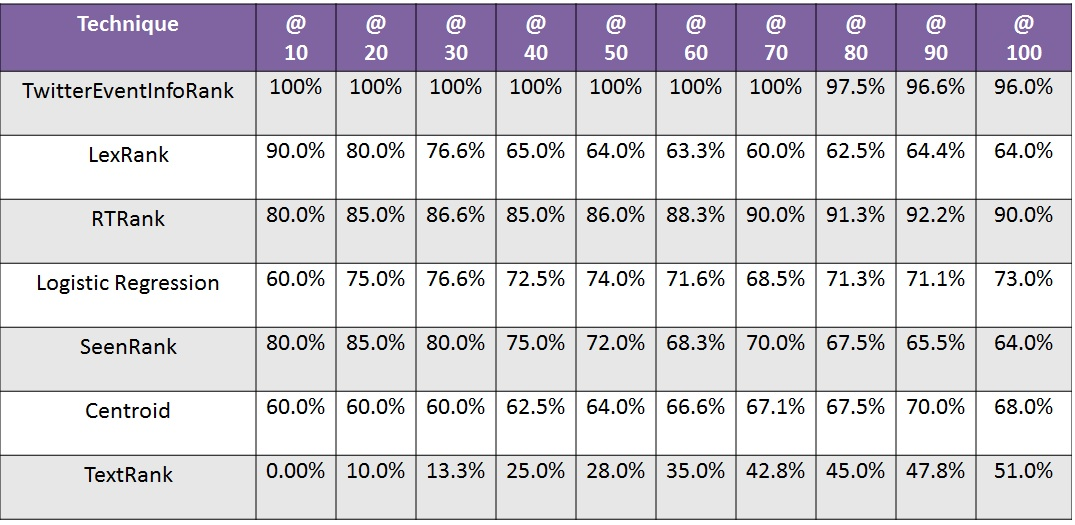
\includegraphics[height=3.5in,width=5.5in]{Figures/millionsmarchnycprecision.jpg}
\caption{\small Performance comparison of ranking techniques using precision scores.}
\label{millionsmarchnycprecision}
\end{figure}

\begin{figure}[htbp]
\centering
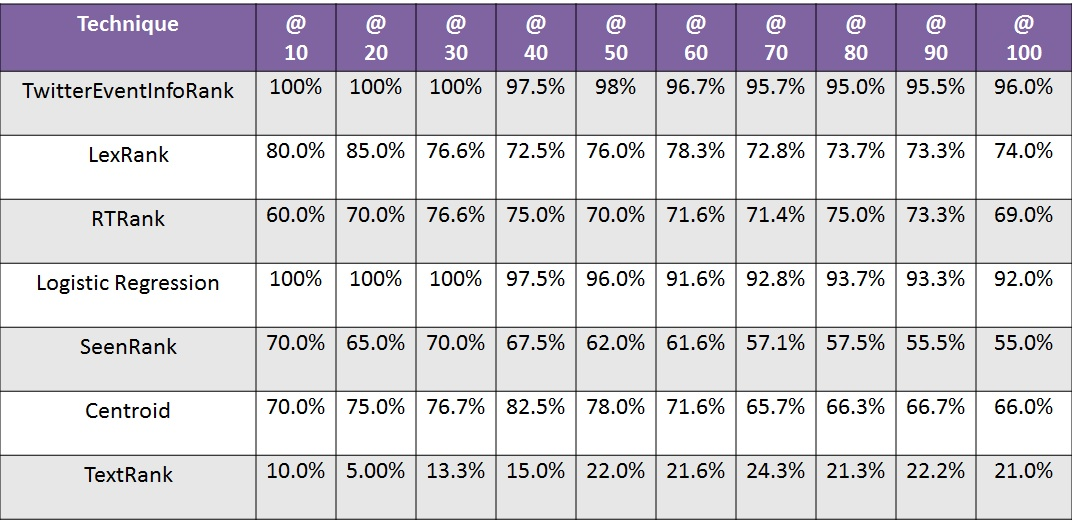
\includegraphics[height=3.5in,width=5.5in]{Figures/sydneysiegeprecision.jpg}
\caption{\small Performance comparison of ranking techniques using precision scores.}
\label{sydneysiegeprecision}
\end{figure}


\section{Event Reference Resolution}

\begin{figure}[htbp]
  \caption{Event Reference Resolution component of the EIIM life cycle.}
  \centering
    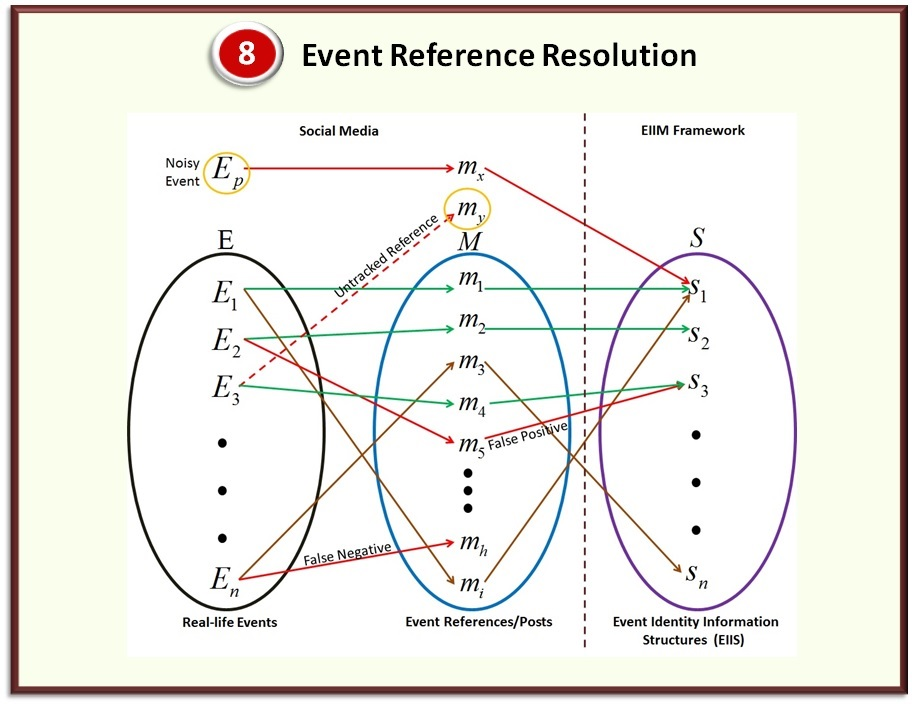
\includegraphics[width=14cm,height=11cm]{Figures/EIIMComponents/EventReferenceResolution.jpg}
\end{figure}

\section{Event Analytics}
\begin{figure}[htbp]
  \caption{Event Analytics component of the EIIM life cycle.}
  \centering
    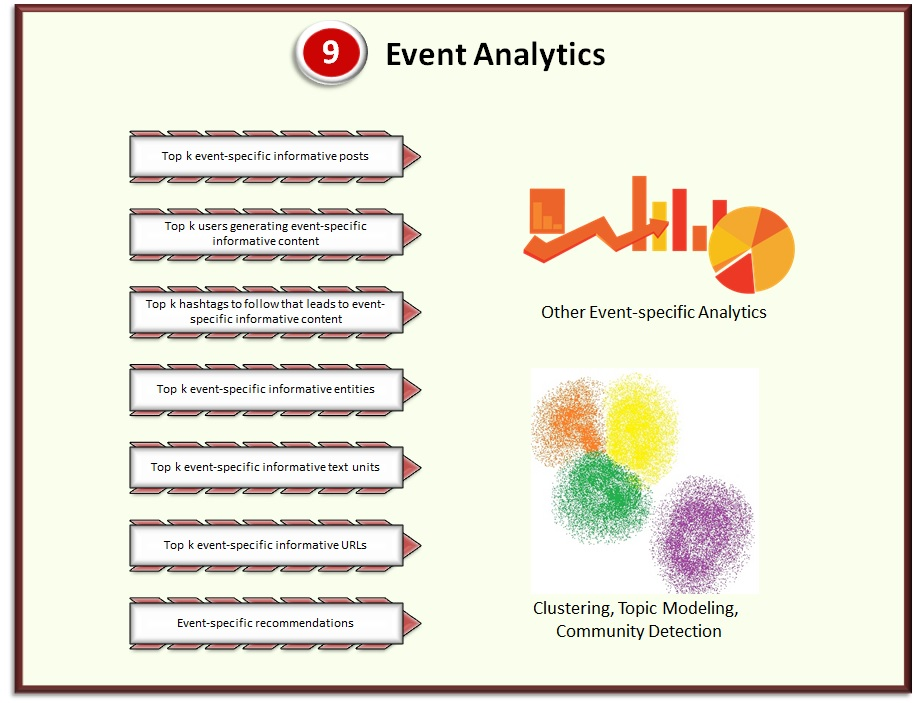
\includegraphics[width=14cm,height=11cm]{Figures/EIIMComponents/EventAnalytics.jpg}
\end{figure}

\paragraph{Top Five Event-specific Informative Hashtags for Sydney Siege Event}
\begin{enumerate}
\item \#sydneysiege 
\item \#SydneySiege
\item \#Sydneysiege
\item \#MartinPlace
\item \#9News                                                                                                                                                                                                                                                                                                                                                                                                                                                                                                                 
\end{enumerate}

\paragraph{Top Five Event-specific Informative Text Units for Sydney Siege Event}
\begin{enumerate}
\item police
\item sydney
\item reporter
\item lindt
\item isis                                                                                                                                                                                                                                                                                                                                                                                                                                                                                                                
\end{enumerate}

\paragraph{Top Five Event-specific Informative URLs for Sydney Siege Event}
\begin{enumerate}
\item http://www.cnn.com/2014/12/15/world/asia/australia-sydney-hostage-situation/\\index.html
\item http://www.bbc.co.uk/news/world-australia-30474089
\item http://edition.cnn.com/2014/12/15/world/asia/australia-sydney-siege-scene/\\index.html
\item http://rt.com/news/214399-sydney-hostages-islamists-updates/ 
\item http://www.newsroompost.com/138766/sydney-cafe-siege-ends-gunman-among-two-killed                                                                                                                                                                                                                                                                                                                                                                                                                                                                                                                
\end{enumerate}

\paragraph{Top Five Event-specific Informative Tweet Excerpts for Sydney Siege Event}
\begin{enumerate}
\item RT @faithcnn: Hostage taker in Sydney cafe has demanded 2 things: ISIS flag and; phone call with Australia PM Tony Abbott \#SydneySiege http://t.co/a2vgrn30Xh
\item Aussie grand mufti and; Imam Council condemn \#Sydneysiege hostage capture http://t.co/ED98YKMxqM - LIVE UPDATES http://t.c...
\item RT @PatDollard: \#SydneySiege: Hostages Held By Jihadis In Australian Cafe - WATCH LIVE VIDEO COVERAGE http://t.co/uGxmd7zLpc \#tcot \#pjnet \\ sydney-siege-scene/index.html
\item RT @FoxNews: MORE: Police confirm 3 hostages escape Sydney cafe, unknown number remain inside http://t.co/pcAt91LIdS \#Sydneysiege
\item Watch \#sydneysiege police conference live as hostages are still being held inside a central Sydney cafe http://t.co/OjulBqM7w2 \#c4news
\end{enumerate}


\paragraph{Three Randomly Selected Tweets for Top Three Event-specific Informative Users posting about Sydney Siege Event.}
\begin{enumerate}
\item \textbf{User 1}
\begin{enumerate}
\item RT @cnni: Hostage taker in Sydney cafe demands ISIS flag and call with Australian PM, Sky News reports. http://t.co/a2vgrn30Xh \#sydneysiege
\item RT @DR\_SHAHID: Hostage taker demands delivery of an \#ISIS flag and a conversation with Prime Minister Tony Abbott http://t.co/xTSDMKCPcD
\item RT @SkyNewsBreak: Update - New South Wales police commissioner confirms five hostages have escaped from the Lindt cafe in Sydney \#sydneysiege
\end{enumerate}

\item \textbf{User 2}
\begin{enumerate}
\item RT @smh: NSW Police Deputy Commissioner Catherine Burn will hold a press conference to update on the \#SydneySiege at 6.30pm.
\item RT @Y7News: Helpful travel advice for commuters heading out of \#Sydney’s CBD this evening - http://t.co/aQx2lvSosm \#sydneysiege
\item RT @hughwhitfeld: British PM David Cameron informed of \#sydneysiege ..UK Foreign Office is in touch with Aus authorities
\end{enumerate}

\item \textbf{User 3}
\begin{enumerate}
\item RT @RT\_com: \#SYDNEY: Gunman tall man in late 40s, dressed in black – eyewitness http://t.co/m51P8dUPhB \#SydneySiege http://t.co/NvJzFsGrFN
\item RT @NewsAustralia: 2GB's Ray Hadley claims hostage takers in \#SydneySiege "wants to speak to Prime Minister Abbott live on radio."
\item RT @BBCWorld: "Profoundly shocking" -Australia PM Tony Abbott delivers second \#sydneysiege statement. MORE: http://t.co/VaKt3ZpRZR
\end{enumerate}

\end{enumerate}

\paragraph{Top Five Event-specific Informative Hashtags for Millions March NYC Event}
\begin{enumerate}
\item \#MillionsMarchNYC
\item \#BlackLivesMatter
\item \#ICantBreathe
\item \#ShutItDown
\item \#millionsmarchnyc                                                                                                                                                                                                                                                                                                                                                                                                                                                                                                                 
\end{enumerate}

\paragraph{Top Five Event-specific Informative Text Units for Millions March NYC Event}
\begin{enumerate}
\item police
\item nyc
\item eric
\item protesters
\item nypd                                                                                                                                                                                                                                                                                                                                                                                                                                                                                                                
\end{enumerate}

\paragraph{Top Five Event-specific Informative URLs for Millions March NYC Event}
\begin{enumerate}
\item http://rt.com/usa/214203-protests-police-brutality-nationwide/\\index.html
\item http://mashable.com/2014/12/13/time-lapse-new-york-protest-march/?utm\_cid=mash-com-Tw-main-link
\item http://www.cbsnews.com/news/eric-garner-ferguson-missouri-protesters-converge-on-washington/
\item http://www.huffingtonpost.com/2014/12/13/millions-march-nyc\_n\_6320348.html?ncid=tweetlnkushpmg00000051 
\item https://www.youtube.com/watch?v=Iz7hkfNmfTY\&feature=youtu.be                                                                                                                                                                                                                                                                                                                                                                                                                                                                                           
\end{enumerate}

\paragraph{Top Five Event-specific Informative Tweet Excerpts for Millions March NYC Event}
\begin{enumerate}
\item RT @rightnowio\_feed: Timelapse video reveals massive size of New York City prot... http://t.co/oHtIhEK969 \#Soho \#Millionsmarchnyc \#NEWYorkC..
\item "@Breaking911: BREAKING NOW: \#NYPD OFFICER INJURED ON THE BROOKLYN BRIDGE BY PROTESTERS THROWING ITEMS AT OFFICERS \#MillionsMarchNYC" Great
\item RT @mohkeit: MT @WSJ: march to NYPD headquarters to protest police brutality \#MillionsMarchNYC http://t.co/zhNSngjbkN http://t.co/YLMJ8uJnJ
\item RT @NaomiCampbell: Peaceful March Saturday Dec 13th Washington Square Park NYC 2:00pm march   Tell everyone U know \#MillionsMarchNYC
\item RT @anregarret: Incredible day! \#MillionsMarchNYC On NYPD Headquarters To Protest Police Killings http://t.co/P2QHvxl9xb via @blackvoices \end{enumerate}

\paragraph{Three Randomly Selected Tweets for Top Three Event-specific Informative Users posting about Millions March NYC Event for a particular hour.}
\begin{enumerate}
\item \textbf{User 1}
\begin{enumerate}
\item RT @mashable: Timelapse video reveals massive size of New York City protests http://t.co/zhqHpkDLk1 \#MillionsMarchNYC http://t.co/WktxssAfDp
\item RT @DahmPublishing: RT@wendycarrillo: Real thugs wear flag pics and Eric Garner's eyes are haunting image \#MillionsMarchNYC http://t.co/7wY…
\item RT @TheRoot: RT @mfmartinez: Protesters continue gathering in Washington Square Park \#MillionsMarchNYC \#TheRootMOW http://t.co/IwkQG1KjFg
\end{enumerate}

\item \textbf{User 2}
\begin{enumerate}
\item RT @roqchams: Thousands march on NYPD headquarters to protest police terrorism http://t.co/yVyUVYkd9X http://t.co/X4QZrfOISh \#MillionsMarchNYC
\item RT @NYjusticeleague: Hundreds killed. Ten Demands. One Continued Fight.  Sign our petition at: http://t.co/KETNo6bS0V \#MillionsMarchNYC htt…
\item RT @cobismith: Union Square now with NYPD in foreground, \#MillionsMarchNYC protesters at right and; US national debt ticker on the left http:/…
\end{enumerate}

\item \textbf{User 3}
\begin{enumerate}
\item RT @mashable: Timelapse video reveals massive size of New York City protests http://t.co/zhqHpkDLk1 \#MillionsMarchNYC http://t.co/WktxssAfDp
\item RT @KeeganNYC: LOTS of NYPD waiting for protesters on the BK side of the Brooklyn Bridge \#MillionsMarchNYC \#ShutItDown \#ICantBreathe http:/…
\item RT @Zegota42: . @KeeganNYC Protesters on Brooklyn Bridge leaving Manhattan Skyline behind. \#MillionsMarchNYC \#ICantBreathe http://t.co/UPvN…
\end{enumerate}

\end{enumerate}


